\section{Theory}
This chapter provides the theoretical background needed to understand the work in this thesis. Beginning with Automatic Train Operation and the role of remote driving within that framework, it covers the fundamentals of video streaming including codecs and transport protocols, introduces GStreamer as the core technology used in the pipeline, describes the main sources of latency in a streaming system, and discusses the relevant characteristics of the communication technologies used in testing.

\subsection{Remote Train Operations}\label{sec:rto}
 
Remote Train Operations (RTO) refer to the act of monitoring and controlling a train from a location outside the locomotive, typically a centralised control room, using live video and a remote control interface. As railways move toward higher levels of automation, RTO has become an important part of safety features and the practical deployment. It allows human operators to intervene when automated systems encounter situations they cannot handle on their own, and it serves as a required fallback layer for trains operating without a driver or staff adequate to drive~\cite{jurgensen2025, fp2r2dato2023d5_4}.
 

\subsubsection{Grades of Automation}\label{subsec:goa}
 
The Grade of Automation (GoA) is a classification system defined in the international standard IEC~62290--1 that describes how much of the train operation is handled automatically instead of by a human~\cite{iec62290}. The standard defines five levels, from GoA~0 to GoA~4, where each higher level adds more responsibility from the driver to the automated system. Table~\ref{tab:goa} summarises the levels.
 
\begin{table}[h]
\centering
\caption{Grades of Automation as defined in IEC~62290--1~\cite{iec62290, uitp2018}.}\label{tab:goa}
    \begin{tabular}{p{1cm} p{3cm} p{8cm}}
    \toprule
    \textbf{GoA} & \textbf{Name} & \textbf{Description} \\
    \midrule
    GoA 0 & On-sight operation   & Fully manual with no automatic protection.\\
    GoA 1 & Manual operation     & Driver controls the train; Automatic Train Protection (ATP) enforces speed limits and safe separation.\\
    GoA 2 & Semi-automated (STO) & ATO handles acceleration and braking; a driver remains on board for doors, obstacle response, and degraded modes.\\
    GoA 3 & Driverless (DTO)     & No driver needed in normal operation. On-board staff may be present for passenger assistance and emergencies. \\
    GoA 4 & Unattended (UTO)     & Fully automatic operation with no staff on board. Remote supervision and control are required for incidents. \\
    \bottomrule
    \end{tabular}
\end{table}
 
RTO is most relevant from GoA~3 upward. At GoA~3, on-board staff can still respond to incidents directly, but remote oversight is used for operational management. At GoA~4, where no staff are on board, RTO becomes the primary mechanism for human intervention when automated systems fail or encounter unexpected conditions~\cite{europesrail2025_d3, orr2024}.
 
\subsubsection{Role of Video in Remote Operation}\label{subsec:video-role}

A remote operator who cannot physically see or hear the train must rely entirely on what the system provides. In practice, this means live video from cameras mounted on or near the train is the most important source of situational awareness~\cite{brandenburger2023, kozarevic2025}. Without a stable and clear video feed, the operator cannot assess track conditions, detect obstacles, interpret signals, or make safe decisions about speed and braking.
 
Research on human factors in remote driving consistently shows that video quality has a direct effect on operator performance. Studies on bitrate, frame rate, and resolution indicate that reductions in bitrate lead to measurable drops in both reaction speed and accuracy, while changes in frame rate have a smaller effect within typical operating ranges~\cite{brandenburger2023}. This suggests that encoding and transmission choices in the video pipeline are not just technical decisions but directly influence operational safety.

Beyond individual video quality, remote train driving typically requires multiple simultaneous camera views. A camera facing straight forward is needed for obstacle and signal detection, while side cameras support the operator's experience, needed for immersiveness of speed and movement like you can see a Figure~\ref{fig:trippelmonitor}~\cite{fp2r2dato2023d5_4, jurgensen2025, neumeier2019}.
 
\begin{figure}[h]
    \centering
    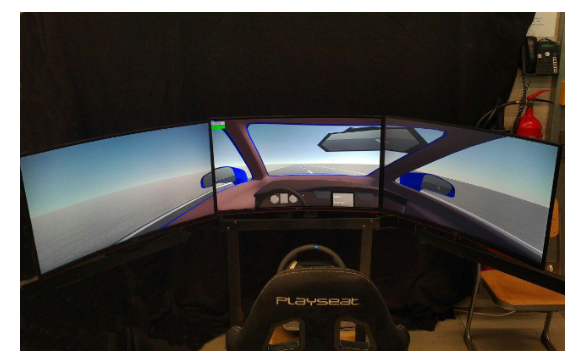
\includegraphics[width=0.6\textwidth]{Images/Theory/ThreeMonitorSetup.png}
    \caption{Three monitor tele operation simulator setup used by Neumeier et al.\ to evaluate the effect of latency on remote driving performance~\cite{neumeier2019}.}\label{fig:trippelmonitor}
\end{figure}

\subsubsection{Latency Requirements and Regulations}\label{subsec:latency-reqs}
 
Latency is a central performance parameter in a RTO video system. If the delay between what happens on the track and what the operator sees on screen is too large, safe intervention becomes impossible. As of now, a big challenge is that no single universally agreed threshold exists for remote train operation, and most values currently used in the field are borrowed from research on cars, drones, and cranes~\cite{myhrvold2025}.
 
The most relevant regulatory reference comes from 3GPP TS~22.289, a technical specification developed in cooperation with the International Union of Railways (UIC) and the European Telecommunications Standards Institute (ETSI)~\cite{3gppts22289}. It classifies remote video control at GoA~3 and GoA~4 as \textit{Very Critical Video Communication} and sets a target end-to-end latency of \(\leq 100\)~ms at speeds up to 500~km/h, or \(\leq 10\)~ms at speeds up to 40~km/h, with a reliability requirement of 99.9\% and a data rate of 10--20~Mbps. These values are defined at the communication interface and are not yet formally adopted into ERA's Technical Specifications for Interoperability (TSIs)~\cite{3gppts22289}.
 
Empirical studies from railway demonstrations report glass-to-glass (G2G) latency values of 340--380~ms for tramway remote driving using commercial systems~\cite{fp2r2dato2024d41_2}, while the Kozarevic study at NTNU measured an average of around 120~ms to 240~ms using a GPS-synchronised measurement method~\cite{kozarevic2025}. Human factors research from other vehicle domains suggests that operators begin to adjust their behaviour at delays above 250--300~ms, and that latency variability can also be more disruptive than a consistently higher but stable delay~\cite{myhrvold2025, neumeier2019}.

\subsection{Video Streaming}\label{sec:video-streaming}
Video streaming is the continuous transmission of video data from a source to a receiver over a network, allowing the receiver to display the content in real time without storing the full recording first~\cite{sodagar2011}. In a remote train operation context, this means live footage from cameras on or near the train is captured, compressed, sent across a network, and displayed on the operator's screen with as little delay as possible.
 
A video streaming system can be thought of as a chain of components, each with its own role. At the sending end, raw video is captured by a camera and handed to an encoder, which compresses it into a format suitable for transmission. The compressed data is then packaged into a transport protocol and sent across the network. At the receiving end, the process is reversed: packets are reassembled, decoded back into raw frames, and rendered on screen. The choices made at each step, which codec, which protocol, which network directly affect the end-to-end latency and video quality that the remote operator experiences~\cite{myhrvold2025, mejias2024}.

\subsection{Video Compression}\label{subsec:codecs}
Video compression works by removing redundancy from the raw video signal. There are two main redundancy that codecs use for compression. Spatial redundancy exists within a single frame where neighbouring pixels often have similar values, as you can see at Figure~\ref{fig:spatial-redundancy} where the background and some of the skin share the same colour. Temporal redundancy exists across frames where much of the image remains unchanged between one frame and the next, as you can see at Figure~\ref{fig:temporal-redundancy} where only the people move, while the background and table stay still. A video encoder exploits both types of redundancy to represent the video with fewer bits than the original raw data. Compression can be lossless where the original data can be perfectly reconstructed, or lossy where some information is discarded in exchange for a much smaller file size. Most video streaming applications use lossy compression, as lossless video requires far more bandwidth than most networks can provide~\cite{blomqvist2018, richardson2010}.

\begin{figure}[h]
    \centering
    \begin{minipage}{0.35\textwidth}
        \centering
        
\includegraphics[width=\textwidth]{Images/Theory/SpatialRed.png}
        \caption{Spatial redundancy~\cite{kondoz2010}.}\label{fig:spatial-redundancy}
    \end{minipage}
    \hfill
    \begin{minipage}{0.6\textwidth}
        \centering
        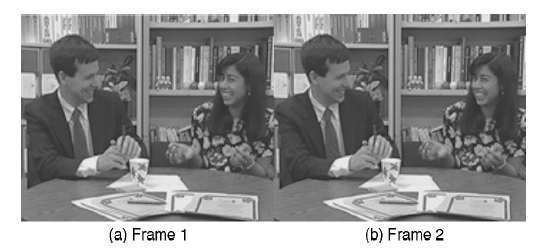
\includegraphics[width=\textwidth]{Images/Theory/TemperoalRed.png}
        \caption{Temporal redundancy~\cite{kondoz2010}.}\label{fig:temporal-redundancy}
    \end{minipage}
\end{figure}

\subsubsection{H.264}\label{subsubsec:h264}
H.264, also known as Advanced Video Coding (AVC), is a video compression standard developed jointly by the ITU-T Video Coding Experts Group and the ISO/IEC Moving Picture Experts Group~\cite{wiegand2003}. It has become the dominant codec for real-time video applications including video conferencing, IP surveillance, and live streaming, due to its balance between compression efficiency, computational cost, and broad hardware support~\cite{sullivan2004}.
 
The codec reduces redundancy across two dimensions. Within a single frame, intra-frame prediction estimates pixel values from neighbouring blocks and stores only the difference. Across consecutive frames, inter-frame prediction identifies how blocks have moved and stores motion vectors rather than full pixel data, allowing H.264 to represent video at significantly lower bitrates than older standards such as MPEG-2 while maintaining comparable visual quality~\cite{wiegand2003}.
 
An important concept is the Group of Pictures (GOP), which defines how often a full intra-coded frame appears in the stream. Short GOP intervals are preferred for real-time applications to reduce both start-up delay and recovery time after packet loss, at the cost of a slightly higher average bitrate~\cite{sullivan2004}. How the encoded data is structured for network transport is described in Section~\ref{subsubsec:nal}.

\subsubsection{H.265}\label{subsubsec:h265}
H.265, also known as High Efficiency Video Coding (HEVC) and formally standardised as ITU-T~H.265 and ISO/IEC~23008--2, is the successor to H.264 published in 2013~\cite{sullivan2012hevc}. Its primary goal was to achieve roughly 50\% better compression compared to H.264 at equivalent visual quality~\cite{ohm2012}.
 
HEVC achieves its efficiency gains by replacing the fixed 16$\times$16 macroblock structure of H.264 with a flexible Coding Tree Unit (CTU) architecture that supports block sizes up to 64$\times$64 pixels as you can see in Figure~\ref{fig:264v265encoding}. Larger blocks handle uniform image regions efficiently, while smaller blocks are used in areas with fine detail or motion. This adaptive structure allows the encoder to allocate coding effort where it is most needed, reducing the total number of bits required to represent a frame at a given quality level~\cite{sullivan2012hevc}.

\begin{figure}[h]
    \centering
    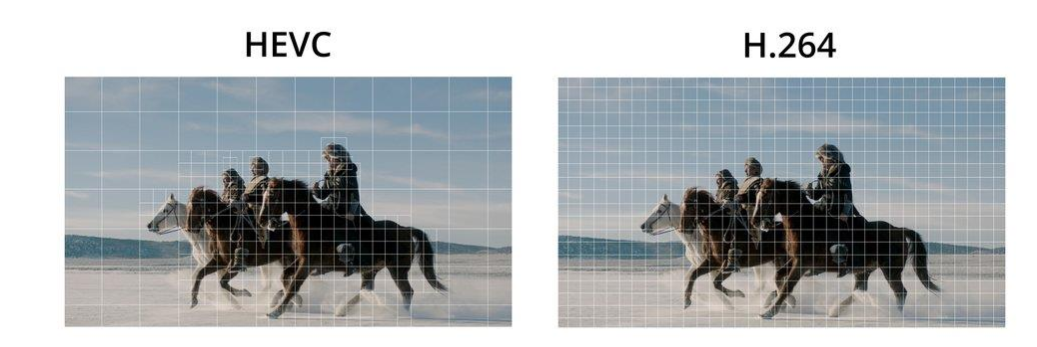
\includegraphics[width=0.8\textwidth]{Images/Theory/264265HEVC.png}
    \caption{Difference between HEVC, H.265 technology, and H.264 of method for encoding~\cite{blomqvist2018}.}\label{fig:264v265encoding}
\end{figure}

Another difference compared to H.264 is computational cost. Encoding with H.265 requires significantly more processing power, which increases encoding time and places greater demand on the sender hardware~\cite{ohm2012}.


\subsubsection{Frame Types}\label{subsubsec:frametypes}

Both H.264 and H.265 organise their compressed video into three frame types, each with a different role in the compression scheme~\cite{seeling2014}.
 
An I-frame, or intra-coded frame, is compressed using only the data within the frame itself, with no reference to any other frame. It can therefore be decoded independently and serves as a recovery point in the stream. A P-frame, or predictive frame, stores only the differences relative to a previously decoded I or P frame, reducing the amount of data needed to represent a frame where little has changed. A B-frame, or bidirectionally predicted frame, can reference both a preceding and a following frame, achieving even higher compression by interpolating between two reference points~\cite{seeling2014}.
 
The sequence of frame types between two consecutive I-frames is called a Group of Pictures (GOP). A shorter GOP means I-frames appear more frequently, which increases the average bitrate but improves the ability to recover from packet loss and reduces the delay before a new receiver can begin decoding the stream.

\subsubsection{NAL Units}\label{subsubsec:nal}
 
Both H.264 and H.265 organise their encoded bitstream through a Network Abstraction Layer (NAL). The NAL divides the encoded data into discrete units called NAL units, each consisting of a header that identifies the type of data it contains, followed by the payload~\cite{wiegand2003}. There are two categories: Video Coding Layer (VCL) NAL units carry the compressed image data, while non-VCL NAL units carry decoder configuration information, most importantly the Sequence Parameter Set (SPS) and Picture Parameter Set (PPS). The SPS contains configuration that applies to the entire video sequence such as resolution and profile, while the PPS contains parameters applying to individual pictures such as entropy coding mode. A decoder must receive both before it can decode any VCL data~\cite{vocal_nal}.
 
When H.264 or H.265 is carried over RTP, each NAL unit is mapped to one or more RTP packets. If a NAL unit exceeds the network maximum transmission unit (MTU), it is fragmented across multiple consecutive RTP packets. The RTP marker bit is set on the last packet of a complete frame, signalling to the receiver that all data for that frame has arrived~\cite{rfc6184}.

\subsubsection{MJPEG}\label{subsubsec:mjpeg}
Motion JPEG (MJPEG) is a video format in which each frame is compressed independently as a JPEG image, with no reference to any other frame in the sequence~\cite{wikipedia_mjpeg}. This purely intraframe approach contrasts with H.264 and H.265, which both rely on temporal prediction across frames to achieve compression.
 
Because each frame carries all the data needed for its own decoding, MJPEG has two notable properties relevant to remote operation. First, packet loss affects only the frame it occurs in, with no propagation of errors to subsequent frames. Second, encoding and decoding complexity is low and predictable, as the encoder processes each frame in isolation without any lookahead or motion estimation~\cite{econ2024}. These properties can result in lower and more consistent encoding latency compared to inter-frame codecs under the same hardware conditions.
 
The main limitation of MJPEG is its high bandwidth consumption. Without temporal compression, every frame must carry its full spatial data, which results in bitrates several times higher than H.264 at equivalent quality~\cite{kaknjo2018videolatency}.

\subsection{Transport Protocols}\label{subsec:transport-protocols}
 
\subsubsection{RTP and SRTP}\label{subsubsec:rtp-srtp}
The Real-time Transport Protocol (RTP) is a network protocol designed for the delivery of audio and video over IP networks, standardised by the IETF in RFC~3550~\cite{rfc3550}. It operates at the application layer and is typically carried over UDP, adding a structured header on top of each media payload. The header contains a sequence number that increments with each packet, allowing the receiver to detect packet loss and reorder out of order arrivals. A timestamp reflects the sampling time of the media content and is used to pace playback at the correct rate on the receiving end. The marker bit signals significant events in the stream, most commonly the last packet belonging to a video frame, so the receiver knows when a complete frame has arrived and is ready for decoding~\cite{rfc3550}.
 
RTP is typically paired with the RTP Control Protocol (RTCP), which runs on a separate port alongside the media stream. RTCP carries periodic reports containing statistics such as packet loss, jitter, and round trip delay, giving both sides visibility into network conditions without carrying any media itself~\cite{rfc3550}.
 
The Secure Real-time Transport Protocol (SRTP) is a security profile built on top of RTP, defined in RFC~3711~\cite{rfc3711}. It adds AES encryption to protect the payload, HMAC authentication to verify packet integrity, and replay protection to reject duplicate packets. Each packet is encrypted independently, so the loss of one packet does not affect the decryption of those that follow. The added overhead per packet is small and the computational cost on modern hardware is low~\cite{rfc3711}.

\subsubsection{UDP}\label{subsubsec:udp}
The User Datagram Protocol (UDP) is a transport layer protocol defined in RFC~768~\cite{rfc768}. It provides a minimal communication mechanism for sending packets, called datagrams, between applications over an IP network. UDP does not establish a connection before sending, makes no guarantee of delivery or packet ordering, and does not retransmit lost packets. Each datagram is handled independently, and the protocol adds only an eight byte header containing source port, destination port, length, and a checksum for basic integrity verification~\cite{rfc768}.
 
The absence of connection setup and retransmission mechanisms means UDP introduces very little overhead and no additional delay beyond the time required to transmit the data itself. This makes it well suited for applications where low latency is more important than guaranteed delivery, such as real-time audio and video streaming, where a retransmitted packet arriving late is less useful than a fresh one~\cite{forouzan2012}.

\subsubsection{TCP}\label{subsubsec:tcp}
The Transmission Control Protocol (TCP) is a transport layer protocol defined in RFC~793~\cite{rfc793}. Unlike UDP, TCP is connection oriented, meaning that a logical connection is established between two endpoints through a handshake process before any data is exchanged. TCP guarantees reliable, ordered delivery by assigning sequence numbers to all transmitted bytes and requiring the receiver to send acknowledgements back to the sender. Any packet that is not acknowledged within a timeout period is retransmitted automatically~\cite{rfc793}.
 
TCP also implements flow control and congestion control mechanisms. Flow control prevents the sender from transmitting data faster than the receiver can process it, using a sliding window that the receiver advertises. Congestion control reduces the transmission rate when packet loss is detected, interpreting loss as a signal of network congestion~\cite{forouzan2012}. These mechanisms make TCP well suited for applications that require complete and correct data delivery, such as file transfer and web browsing, but the added overhead means the transmission rate can vary depending on network conditions~\cite{forouzan2012}.

\subsection{Streaming Parameters}\label{subsec:streaming-params}
 
\subsubsection{Bandwidth}\label{subsubsec:bandwidth}
Bandwidth in video streaming refers to the amount of data that can be transmitted per unit of time across a network connection, typically measured in megabits per second (Mbps). In a streaming pipeline the term bitrate is often used alongside bandwidth: bitrate describes how much data the encoder produces per second, while bandwidth describes how much the network can carry. When bitrate exceeds available bandwidth, packets accumulate in buffers or are dropped, leading to increased latency, visual degradation, or stream interruptions~\cite{sodagar2011}.
 
The required bandwidth depends on the codec, resolution, frame rate, and scene complexity. A higher bitrate generally produces better visual quality, but the relationship is not linear. Subjective testing has shown that perceived quality improves sharply at low bitrates and then levels off as bitrate increases, meaning that doubling the bitrate does not double the perceived quality~\cite{pinson2012}.
 
\subsubsection{Resolution}\label{subsubsec:resolution}
 
Resolution defines the number of pixels in each video frame, expressed as width by height. Common values include 1280$\times$720 (720p) and 1920$\times$1080 (1080p). A higher resolution captures more spatial detail, but also increases the amount of data per frame that the encoder must compress and the network must carry~\cite{pinson2012}.
 
For a given codec and bitrate, increasing resolution without increasing the bitrate results in more compression per pixel, which can reduce sharpness and introduce visible artefacts. Conversely, a high resolution with a sufficiently high bitrate produces a clearer image. The 3GPP Rel-16 specification for video based remote railway control recommends a minimum of 1920$\times$1080 at 30 frames per second as the target output quality~\cite{mejias2024}.

% ─────────────────────────────────────────────────────────────────────────────

\subsection{Latency Sources in a Video Streaming Pipeline}\label{sec:latency-sources}
The total delay from when a video frame is captured by a camera to when it is displayed on the operator's screen is commonly referred to as glass-to-glass latency. This delay does not originate from a single component but accumulates across each stage of the streaming pipeline~\cite{dobrian2011}. Understanding where latency is introduced at each stage is necessary for identifying bottlenecks and evaluating the overall performance of a streaming system.
 
The pipeline can be divided into five sequential stages: capturing, encoding, transmitting, decoding, and rendering. Each stage contributes a portion of the total delay, and the contribution of each depends on the hardware, configuration, and network conditions in use~\cite{kaknjo2018}. The following subsections describe each stage and the mechanisms through which latency is introduced.

\subsubsection{Capturing}\label{subsec:capturing}
Capturing latency is the delay introduced at the camera before any data enters the network pipeline. It originates from two main sources: the exposure time of the image sensor and the subsequent image processing performed inside the camera~\cite{axis2024}.
 
The image sensor captures light across all its pixels during one exposure interval before converting the accumulated light energy into digital signals. At 30 frames per second the sensor collects light for approximately 33 milliseconds per frame, meaning that any event occurring just after the start of an exposure interval must wait until the end of that interval before it is registered~\cite{axis2024}. Higher frame rates reduce this waiting time proportionally.
 
After exposure, the raw sensor data passes through a series of internal processing steps such as demosaicing, noise reduction, and scaling before being handed to the encoder. The time required for these steps depends on the camera hardware and the features enabled, and can add several milliseconds to the total capture delay~\cite{axis2024, kaknjo2018}. In network cameras the combined capture and internal processing time is typically under 50 milliseconds, though it varies between camera models and frame types.

 
\subsubsection{Encoding}\label{subsec:encoding}
Encoding latency is the delay introduced while the encoder compresses raw video frames into a transmittable format. It originates from the computational steps required to apply intra and inter frame prediction, transform coding, and entropy coding to each frame~\cite{axis2024}.
 
Buffering is another significant source of encoding delay. Encoders that use B-frames must hold one or more future frames in memory before the current frame can be encoded, since B-frames reference both past and future frames. This lookahead buffering adds at least one frame period of delay before any data can be output~\cite{hamidouche2022}. Encoders configured for low latency operation typically disable B-frames and lookahead to eliminate this waiting time, at the cost of some compression efficiency.
 
The computational load of the encoding process itself also contributes to delay. More complex encoding settings produce better compression but require more processing time per frame. When the encoding time for a single frame exceeds the frame period, frames begin to queue and latency accumulates over time. The choice of encoder preset and hardware therefore directly affects how much delay the encoding stage adds to the pipeline~\cite{axis2024}.

 
\subsubsection{Transmitting}\label{subsec:transmitting}
Transmission latency is the delay introduced while encoded video data travels across the network from the sender to the receiver. It consists of several components that accumulate along the path~\cite{forouzan2012}.
 
Propagation delay is the time required for a signal to travel physically from the sender to the receiver, determined by the distance between the two endpoints and the speed of signal propagation through the medium. Serialisation delay is the time required to place all the bits of a packet onto the transmission link, determined by packet size and link capacity. Queuing delay occurs when packets wait in buffers at intermediate nodes, such as routers and switches, before being forwarded. In congested networks this can vary considerably from packet to packet~\cite{forouzan2012}.
 
Variation in the arrival time of packets at the receiver is called jitter. When packets that were sent at regular intervals arrive with uneven spacing, the receiver cannot immediately display them in order. To compensate, a jitter buffer is used on the receiver side to hold incoming packets briefly and release them at a steady rate. While this smooths out the stream, the jitter buffer itself introduces additional fixed delay. A larger buffer tolerates more jitter but increases the total latency, while a smaller buffer reduces delay at the cost of being more sensitive to network variation~\cite{axis2024}.

 
\subsubsection{Decoding}\label{subsec:decoding}
Decoding latency is the delay introduced while the receiver decompresses incoming NAL units back into raw video frames for display. The computational steps involved are the inverse of encoding, including entropy decoding, inverse transform, and motion compensation, and their cost depends on the codec and the hardware available~\cite{hamidouche2022}.
 
Frame reordering is another notable source of decoding delay. When B-frames are present in the stream, the decoder receives frames in a different order than they are to be displayed, since B-frames reference future frames that have not yet been decoded. The decoder must therefore buffer frames until their reference frames arrive before it can output them in the correct display order. The number of frames that must be held in this decoded picture buffer (DPB) depends on the GOP structure used by the encoder~\cite{hamidouche2022}.
 
When the encoder is configured without B-frames, as is common in low latency streaming, the reordering delay is eliminated and the decoder can output each frame as soon as it is decoded. The remaining decoding latency is then primarily determined by the processing time per frame, which on modern hardware is typically in the range of a few milliseconds~\cite{axis2024}.

\subsubsection{Rendering}\label{subsec:rendering}
Rendering latency is the delay introduced at the final stage of the pipeline, where a decoded frame is passed to the display and made visible to the viewer. It consists of two main components: the time required for the rendering application to prepare and present the frame to the graphics system, and the time the display itself takes to show it~\cite{axis2024}.
 
A display can only update its image at the rate defined by its refresh rate, measured in hertz. A monitor running at 60~Hz updates 60 times per second, meaning a new image appears at most once every 16.7~milliseconds. If a decoded frame arrives just after a refresh has occurred, it must wait until the next refresh cycle before it becomes visible, introducing up to one full frame period of additional latency~\cite{leray2018}. Higher refresh rates reduce this waiting time, as the interval between refresh cycles is shorter.
 
The rendering application may also hold frames in a buffer before handing them to the display, either to synchronise with the refresh cycle or to ensure smooth playback. This buffering adds a predictable but fixed amount of delay. Combined with the display's own internal processing time, rendering latency is typically in the range of one to two frame periods and represents the last contribution to the total glass-to-glass delay~\cite{axis2024}.

 
% ─────────────────────────────────────────────────────────────────────────────

\subsection{Clock Synchronisation}\label{subsec:clock-sync}

Accurate latency measurement between two separate machines requires that both share a common time reference. Each computer maintains an internal clock driven by a local hardware oscillator. Even at identical nominal frequencies, two independent oscillators will accumulate a growing offset over time due to differences in temperature, aging, and manufacturing tolerances~\cite{vannicola2012}. When a timestamp recorded on one machine is compared against a timestamp recorded on another, any offset between the two clocks appears directly in the measured result. Depending on the magnitude of the drift, this error can easily exceed the latency values being measured, making clock synchronisation a requirement for accurate one-way delay measurement.

\subsubsection{GPS-Based Clock Synchronisation}\label{subsubsec:gps-sync}

The Global Positioning System (GPS) operates satellites that each carry onboard atomic clocks traceable to Coordinated Universal Time (UTC). Each satellite broadcasts a navigation message containing the current time along with parameters allowing a receiver to compute the signal propagation delay from the satellite to the receiver. By combining signals from at least four satellites and solving for the receiver position and clock offset simultaneously, a GPS receiver can derive a precise absolute time reference~\cite{misra2011}.

A common timing output from GPS receivers is the pulse-per-second (PPS) signal. This is a periodic electrical pulse whose rising edge is aligned to the UTC second boundary. Commercial GPS receivers designed for timing applications typically achieve a PPS accuracy of 100 nanoseconds or better relative to UTC, and precision timing receivers can reach the range of tens of nanoseconds under stable conditions~\cite{vannicola2012, sesia2010}. The PPS signal provides a hardware-level time reference that is independent of network conditions and available continuously as long as the receiver has a clear view of the sky.

When a computer's operating system is disciplined by a GPS PPS signal, the kernel timestamps each incoming pulse and uses the known UTC alignment to adjust the phase and frequency of the system clock continuously. The resulting clock closely tracks UTC, with residual errors typically in the sub-microsecond range~\cite{sesia2010}. For latency measurements in a video streaming system where delays are on the order of tens to hundreds of milliseconds, this accuracy level means that clock error contributes negligibly to the measured values. GPS-based synchronisation is therefore used in studies where high measurement precision is required and where both endpoints can be equipped with a GPS receiver, as seen in the latency measurement work of Kaknjo et al.~\cite{kaknjo2018} and the tramway remote driving tests reported in FP2R2DATO D41.2~\cite{fp2r2dato2024d41_2}.

\subsubsection{Network-Based Clock Synchronisation with Chrony}\label{subsubsec:chrony-sync}

When a hardware GPS reference is not available, clock synchronisation can be achieved over a network using the Network Time Protocol (NTP). NTP operates by exchanging timestamped packets between a client and one or more time servers. The client records the time it sent the request, the time the server received it, the time the server sent its reply, and the time the client received the reply. From these four timestamps, NTP estimates the round-trip propagation delay and uses half of that value to approximate the one-way delay, computing a correction to the local clock~\cite{rfc5905}.

Chrony is an NTP implementation for Linux systems that is designed to maintain accurate synchronisation under variable network conditions. Rather than making abrupt step corrections to the clock, Chrony adjusts the frequency of the local oscillator continuously, which reduces disruption to running processes and improves long-term stability~\cite{chronyproject}. It also tracks the estimated error of each configured time source and selects the most reliable one based on a combination of stratum, distance, and measured jitter.

When synchronised to public internet time servers such as those provided by the \texttt{pool.ntp.org} project, Chrony typically achieves a clock accuracy within a few milliseconds over an internet connection. On a local area network under stable conditions the accuracy improves to tens of microseconds, and with hardware timestamping enabled on the network interface, where the network card rather than the kernel records packet arrival and departure times, sub-microsecond accuracy is possible~\cite{redhat2024chrony, redhat2024hw}.
% ─────────────────────────────────────────────────────────────────────────────

\subsection{GStreamer}\label{sec:gstreamer}
GStreamer is an open source multimedia framework written in C that allows developers to construct pipelines of media processing components~\cite{gstreamer_intro}. It was originally developed at the Oregon Graduate Institute in 1999 and has since become a widely used foundation for applications ranging from media playback and transcoding to real-time video streaming and computer vision~\cite{gstreamer_intro}. The framework is built around a modular, plugin based architecture where each processing step is provided by a plugin, and individual components can be combined freely to form a complete processing chain suited to the application at hand.
 
The following subsections describe the core concepts of GStreamer that are relevant to understanding how a streaming pipeline is constructed and instrumented.

 
\subsubsection{Pipeline and Elements}\label{subsec:pipeline-elements}
An element is the fundamental building block in GStreamer. Each element performs a single, specific task in the media processing chain, such as reading data from a network socket, decoding a compressed video stream, converting a pixel format, or writing frames to a display. Elements are linked together in sequence to form a pipeline, where the output of one element flows into the input of the next~\cite{gstreamer_elements}.
 
A pipeline is a specialised container that manages a group of connected elements and coordinates their execution. It provides a shared clock that all elements use to synchronise data, and it handles state transitions for the entire graph as a unit. The three main operational states are NULL, PAUSED, and PLAYING.\@In the PLAYING state, data flows continuously from source elements through any intermediate processing elements and finally into sink elements~\cite{gstreamer_elements}.
 
Elements are broadly categorised by their role in the pipeline. Source elements produce data and have no input, for example by reading from a camera or a network port. Filter elements receive data, process it, and pass it on, covering tasks such as encoding, decoding, and format conversion. Sink elements consume data at the end of the pipeline and have no output, typically by rendering video to a screen or writing data to a socket~\cite{gstreamer_elements}. By combining elements of these three types, a complete media processing pipeline can be assembled from reusable components without writing the processing logic from scratch.

 
\subsubsection{Pads}\label{subsec:pads}
Pads are the connection points through which data flows between elements in a GStreamer pipeline. Every element exposes one or more pads, and data moves from the source pad of one element to the sink pad of the next. Source pads produce data and sink pads consume it, where the terms are defined from the perspective of the element itself~\cite{gstreamer_pads}.
 
Each pad carries capability information, called caps, which describes the type and format of data it can handle. This includes properties such as media type, codec, resolution, and frame rate. Before two pads can be linked, GStreamer negotiates a common format by finding the intersection of their capabilities. If no common format exists the link is rejected, preventing incompatible elements from being connected~\cite{gstreamer_pads}.
 
Pads can be either static or dynamic. Static pads are always present on the element from the moment it is created. Dynamic pads appear only when the element begins processing data and has determined what format it is working with, which is common in demuxers and parsers that must read the stream before knowing its structure~\cite{gstreamer_pads}.

 
\subsubsection{Sinks}\label{subsec:sinks}
A sink element is the terminal point of a GStreamer pipeline. It receives data from upstream elements and delivers it to an output destination, such as a display, a file, or a network socket. Sink elements have one or more sink pads for receiving data but no source pads, as they do not pass data further down the pipeline~\cite{gstreamer_sink}.
 
Sink elements are treated specially by the GStreamer core in relation to synchronisation. When a pipeline transitions to the PAUSED state, the sink waits to receive the first buffer or event before confirming the state change. This behaviour allows the pipeline to ensure that data is available and properly configured before playback begins~\cite{gstreamer_sink}.
 
A common type of sink in video pipelines is a display sink, which renders decoded frames to a screen. GStreamer provides several display sink implementations suited to different platforms and windowing systems. The \texttt{sync} property controls whether the sink waits for the correct presentation time before displaying each frame. Setting \texttt{sync=false} disables this waiting and causes the sink to display frames as soon as they arrive, which reduces latency at the cost of ignoring the stream's timing information~\cite{gstreamer_sink}.

\subsubsection{Probes}\label{subsec:probes}
Probes are callbacks that an application can attach to a pad in order to monitor or intercept the data flowing through it at runtime. They allow the application to observe buffers, events, and queries as they pass through a specific point in the pipeline without modifying the pipeline structure itself~\cite{gstreamer_probes}.
 
A probe is installed on a pad using the \texttt{gst\_pad\_add\_probe} function, which accepts a probe type mask and a callback function. The type mask specifies what the probe should respond to, such as the arrival of a buffer, a buffer list, or an event. Each time data matching the type mask passes through the pad, GStreamer calls the registered callback function and passes the data to it. The callback can inspect the data, read timestamps, extract header information, and return a value indicating whether the data should continue flowing, be dropped, or cause the pad to block~\cite{gstreamer_probes}.
 
Probes are particularly useful for latency measurement, as they allow the application to record a timestamp at one pad when data enters the pipeline and another timestamp at a downstream pad when the processed data exits. The difference between the two timestamps represents the processing time between those two points in the pipeline~\cite{gstreamer_pipeline_manip}.

% ─────────────────────────────────────────────────────────────────────────────

\subsection{Network and Communication}\label{sec:network}
The network connecting between the sender and receiver is an important part of any remote operation system. The choice of network technology affects how much data can be sent, how quickly it arrives, and how stable the connection is under varying conditions. The following subsections cover the network technologies relevant to this thesis.
 
\subsubsection{Wi-Fi}\label{subsec:wifi}
Wi-Fi is a family of wireless networking technologies based on the IEEE 802.11 standard. It allows devices to communicate over a local area network using radio frequencies, most commonly 2.4~GHz and 5~GHz~\cite{ieee80211}. The 2.4~GHz band covers longer distances but offers lower maximum data rates, while the 5~GHz band supports higher data rates over shorter distances.
 
Wi-Fi networks operate on unlicensed radio channels where all nearby devices transmit on the same frequency. When multiple devices transmit at the same time, collisions occur and data must be retransmitted. This can increase latency and reduce predictability, particularly when the network is busy~\cite{bankov2019}. For controlled environments with few devices, Wi-Fi can deliver low and stable latency.

\subsubsection{Cellular and 5G}\label{subsec:5g}
Cellular networks provide wireless communication over wide areas by dividing coverage into cells, each served by a base station. Data travels from a device through the radio access network to a core network and then on to its destination. Each of these steps adds some delay, and the total latency depends on the network generation, radio conditions, and distance to the core~\cite{li2018urllc}.
 
The fifth generation (5G) of cellular networks was designed to support three broad service categories. Enhanced Mobile Broadband (eMBB) targets high data rates for applications such as video streaming. Massive Machine Type Communications (mMTC) connects large numbers of low power devices. Ultra Reliable Low Latency Communications (URLLC) is the category most relevant to remote control, aiming for end-to-end latency below 1~ms and a reliability of 99.999\%~\cite{li2018urllc, schulz2017urllc}. To achieve this, 5G NR introduced a shorter transmission time interval compared to 4G LTE, allowing the network to send and acknowledge data more frequently.
 
In practice, the latency experienced by an application over a 5G network is higher than the theoretical URLLC targets, as it also includes processing in the radio hardware, the core network, and the application itself. Studies on remote vehicle control show that total end-to-end video latency over 5G is typically in the range of tens to a few hundred milliseconds depending on the system architecture, with 5G consistently outperforming 4G in both average latency and stability~\cite{ouden2022}.
 
\subsubsection{Tailscale}\label{subsec:tailscale}
Tailscale is a networking tool that creates a private mesh network between devices over the internet. It is built on top of WireGuard, an open source VPN protocol that uses modern cryptography to establish encrypted tunnels between devices~\cite{tailscale_what}. Each device on the network gets a stable private IP address and can communicate directly with any other device on the same network, regardless of where they are physically located or what network they are connected to.
 
The main idea behind Tailscale is that devices connect directly to each other rather than routing all traffic through a central server. A coordination server handles authentication and helps devices find each other, but once a connection is established the data flows directly between the two endpoints~\cite{tailscale_what}. If a direct connection is not possible due to network restrictions, Tailscale falls back to relay servers to keep traffic flowing.
 
WireGuard, which handles the actual data transfer, adds encryption and authentication to every packet passing through the tunnel. The protocol is designed to have low overhead compared to older VPN technologies, which keeps the additional latency introduced by the encrypted tunnel small~\cite{donenfeld2017wireguard}.

 
% ─────────────────────────────────────────────────────────────────────────────

\subsection{Performance Metrics}\label{sec:metrics}
Evaluating a video streaming system requires measuring several aspects of its behaviour under different conditions. The metrics covered in this section are latency, packet loss, throughput, CPU usage, and visual quality. Together they give a picture of how the system performs from both a network and a visual standpoint.

\subsubsection{Latency}\label{subsec:latency-metric}
Latency in a video streaming system is the time it takes for data to travel from one point to another. The most complete measure is glass-to-glass latency, which covers the full path from when a camera captures an image to when it appears on the operator's screen~\cite{kaknjo2018}. However, glass-to-glass latency alone does not reveal where in the pipeline the delay originates. For this reason it is common to break the total latency into smaller segments that can each be measured independently.
 
Three segments are useful for understanding a streaming pipeline. Sender pipeline latency covers the time from when raw video enters the sender until encoded packets leave it. Transit latency covers the time packets spend travelling across the network. Receiver pipeline latency covers the time from when packets arrive until the decoded frame is ready for display~\cite{kaknjo2018}.
 
There are several ways to measure each segment, and the choice of method has a large impact on the results. As discussed in~\cite{myhrvold2025}, the literature uses a wide range of approaches including round-trip time, one-way delay, and glass-to-glass timing. Round-trip time does not require clock synchronisation but measures both directions combined and cannot separate sender and receiver contributions~\cite{rfc3550}. One-way delay gives a more precise picture of a single direction but requires both endpoints to share a common time reference, as any clock offset between the two machines will appear as measurement error~\cite{kaknjo2018}. NTP can synchronise clocks to within a few milliseconds, while PTP achieves sub-millisecond accuracy with the right network hardware~\cite{rfc3550}. For transit latency, RTP sequence numbers provide a practical basis for measurement, as sender and receiver logs can be compared after a test to reconstruct the timing of individual packets~\cite{rfc3550}.

\subsubsection{Packet Loss}\label{subsec:packet-loss}
Packet loss occurs when one or more packets sent across a network fail to reach the receiver. In UDP based video streaming, lost packets are not retransmitted, so any data they carried is gone. For video encoded with inter-frame prediction, a lost packet can corrupt not only the frame it belongs to but also subsequent frames that reference it, until the next I-frame arrives and allows the decoder to recover~\cite{calyam2012}.
 
Packet loss is most commonly expressed as a percentage of the total packets sent. RTP provides a direct way to detect loss, since the sequence number in each RTP packet increments by one for every packet sent. A receiver can therefore identify a lost packet whenever it observes a gap in the sequence of received numbers~\cite{rfc3550}. The packet loss rate can then be calculated by comparing the number of expected packets, derived from the sequence number range, with the number actually received.
 
Even small amounts of packet loss can have a noticeable effect on video quality. Research on H.264 and H.265 video streams shows that loss rates as low as 0.1\% can produce visible artefacts, and that the effect becomes more severe at higher loss rates and higher resolutions~\cite{pekec2023}.
 
\subsubsection{Throughput}\label{subsec:throughput}
Throughput is the amount of data successfully transmitted from one point to another over a given period of time, measured in bits per second~\cite{forouzan2012}. It describes the actual data transfer rate observed during operation, as distinct from bandwidth, which represents the maximum capacity of the link. Throughput is always equal to or lower than bandwidth, as it is affected by overhead, congestion, and packet loss~\cite{forouzan2012}.
 
In a video streaming context, throughput reflects how much encoded video data is leaving the sender and reaching the network per second. Monitoring throughput over time shows whether the sender is transmitting at a consistent rate and whether the output matches the target bitrate set by the encoder. Variations in throughput can indicate congestion on the network or changes in the encoder output caused by scene complexity~\cite{sodagar2011}.

\subsubsection{CPU Usage}\label{subsec:cpu}
CPU usage is the percentage of time a processor spends actively running instructions during a given measurement interval, as opposed to sitting idle~\cite{linode_sar}. It is typically reported as an average across all cores or per individual core, and is measured continuously to capture how load varies over time.
 
In a video streaming pipeline, the most CPU intensive task on the sender side is encoding. The computational load depends on the codec, the encoder settings, the resolution, and the number of streams being processed simultaneously. When CPU usage remains consistently high, the encoder may not be able to process frames fast enough to keep up with the incoming video rate, which can cause frames to queue and latency to increase~\cite{richardson2010}.
 
CPU usage is commonly measured using system monitoring tools that read data from the operating system at regular intervals. On Linux systems, the \texttt{sar} utility from the \texttt{sysstat} package is a standard tool for this purpose. It samples CPU activity at a set interval and reports metrics such as the percentage of time spent in user space, kernel space, and idle~\cite{linode_sar}.
 
\subsubsection{Visual Quality}\label{subsec:visual-quality}
Visual quality in a video streaming context refers to how well the content received at the display represents what was originally captured. Compression, packet loss, and network conditions can all introduce artefacts such as blocking, blurring, or pixelation that reduce the clarity of the image~\cite{pekec2023}.
 
Image quality assessment (IQA) methods are used to measure these effects in a consistent and repeatable way. They fall into two broad categories. Full reference methods compare a received image against an original, undistorted reference image. Common examples are Peak Signal to Noise Ratio (PSNR) and the Structural Similarity Index (SSIM), both of which quantify the difference between the two images using pixel level calculations~\cite{sara2019}. These methods require access to the original image, which is not always available in a live streaming scenario.
 
No reference methods, also called blind quality assessment, estimate quality from the received image alone without any original to compare against~\cite{mittal2012}. One well established no reference metric is the Blind/Referenceless Image Spatial Quality Evaluator (BRISQUE), proposed by Mittal et al.~\cite{mittal2012}. BRISQUE analyses the statistical properties of the image using a model of how natural, undistorted images are expected to look. When an image contains distortions such as blur, noise, or compression artefacts, its statistical properties deviate from those of a natural image. BRISQUE quantifies this deviation and outputs a score between 0 and 100, where lower scores indicate better quality and higher scores indicate more visible distortion  as you can see in Figure~\ref{fig:brisqueResult}. The model was trained on a dataset of human quality ratings and is designed to correlate with how a human observer would rate the image~\cite{mittal2012}. BRISQUE has been confirmed in practice by Pennada et al.\ that found that images with lower BRISQUE scores consistently achieved higher AI classification accuracy, demonstrating that the metric reliably reflects the kind of quality degradation that affects downstream tasks~\cite{pennada2023}.

\begin{figure}[H]
    \centering
    
\includegraphics[width=0.8\textwidth]{Images/Theory/BRISQUEResult.png}
    \caption{Difference of BRISQUE evaluation~\cite{pennada2023}.}\label{fig:brisqueResult}
\end{figure}

